\documentclass[../manuale-sviluppatore.tex]{subfiles}

\begin{document}
\subsection{Visione generale}
Il plug-in è costituito da un'applicazione per la piattaforma grafana basata sul framework React. Tale componente software riceve in input i dati del predittore, risultato dell'esecuzione della training app su un set di dati di train; in base a questi dati elabora la predizione sui dati attuali ricevuti da Grafana, e visualizza successivamente tale predizione in forma di grafico. \\
Il componente software in oggetto si divide quindi in tre parti principali, che sono:
\begin{itemize}
  \item Il plug-in;
  \item La piattaforma Grafana;
  \item \glossario{InfluxDB}.
\end{itemize}

I tre componenti sono in stretta relazione tra loro; le interazioni che sussistono tra le parti citate sono le seguenti:
\begin{itemize}
  \item InfluxDB, un database di tipo \glossario{time-series}, immagazina i dati su cui è necessario effettuare la predizione;
  \item La piattaforma Grafana si occupa di prelevare i dati su cui effettuare la predizione dal database Influx, e fornirli al plug-in;
  \item Il plug-in, ospitato dalla piattaforma Grafana, si occupa di elaborare i dati forniti da Grafana con gli opportuni algoritmi di predizione, e successivamente di visualizzarli in un opportuno grafico.
\end{itemize}

L'intero plug-in è sviluppato col \glossario{framework} ReactJS; viene usato il pattern architetturale MVC (\textit{model-view-controller}) per la gestione dell'input dei dati dalla componente back-end di Grafana, per la loro elaborazione tramite algoritmi di Regressione Lineare e Support Vector Machines e per il conseguente output a schermo tramite grafico. \\
Viene invece utilizzato il design pattern Strategy per fornire un ulteriore livello di astrazione ai metodi di predizione tramite Regressione Lineare e Support Vector Machines.

\begin{figure}[H]
  \centering
  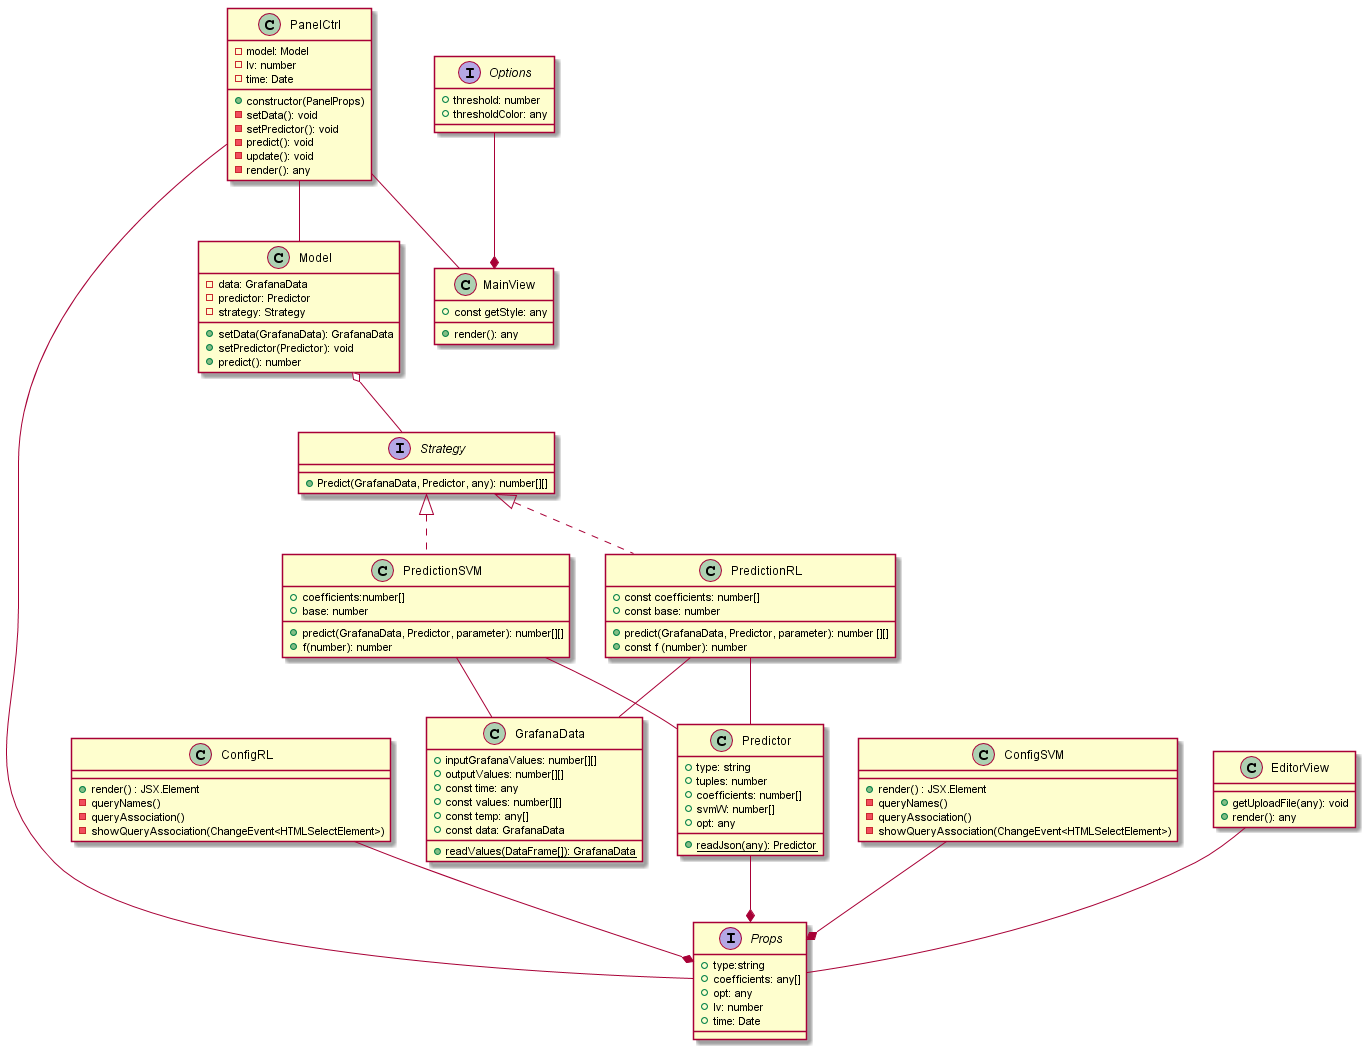
\includegraphics[width=15cm]{img/plugin/GrafanaClasses.png}
  \caption{Diagramma delle classi del plug-in.}
\end{figure}

\begin{figure}[H]
  \centering
  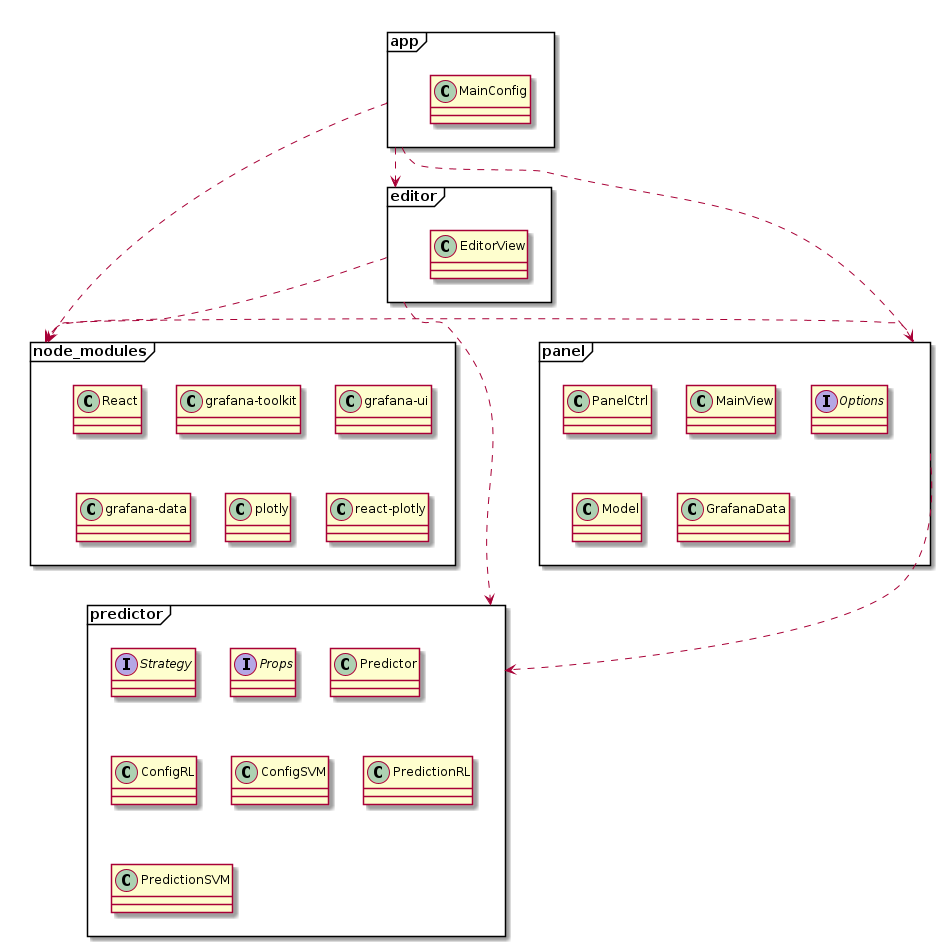
\includegraphics[width=15cm]{img/plugin/packagesDiagramPlug.png}
  \caption{Diagramma dei package del plug-in.}
\end{figure}

\subsection{Design Pattern - MVC}
Il design MVC viene utilizzato per la gestione dell'input dei dati dalla componente back-end di Grafana, per la loro elaborazione tramite algoritmi di Regressione Lineare e Support Vector Machines e per il conseguente output a schermo tramite grafico. Le classi appartenenti a questo design pattern sono PanelCtrl, Model e MainView. \\
La classe PanelCtrl si occupa di impostare i dati di input e il predittore; a partire da questi gestisce la predizione. Essa istanzia inoltre il model, il quale si occupa di reperire i dati da Grafana e il predittore dall'input dell'utente. Questi vengono quindi restituiti al controller, il quale istanzia la classe MainView per la visualizzazione del grafico.

\begin{figure}[H]
  \centering
  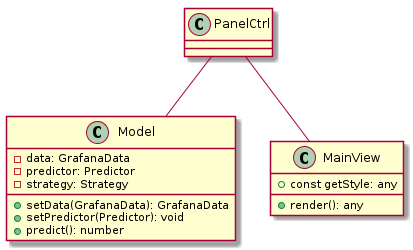
\includegraphics[width=10cm]{img/plugin/mvcplugin.png}
  \caption{Implementazione MVC del plug-in.}
\end{figure}

\subsection{Design Pattern - Strategy}
Viene utilizzato il design pattern Strategy per fornire un ulteriore livello di astrazione ai metodi di predizione tramite Regressione Lineare e Support Vector Machines.
A tale scopo è presente un'interfaccia Strategy che si occupa di eseguire i calcoli interfacciandosi alle classi ConfigRL e PredictionRL per la Regressione Lineare,
o i metodi ConfigSVM e PredictionSVM per le Support Vector Machines. \\

\begin{figure}[H]
  \centering
  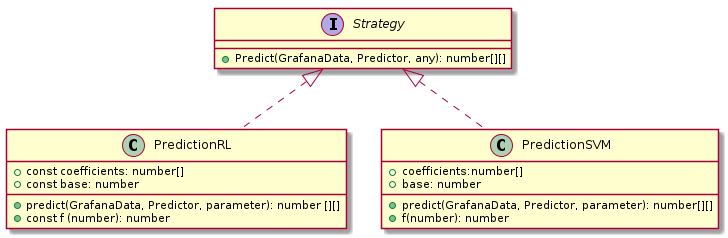
\includegraphics[width=10cm]{img/plugin/strategy.png}
  \caption{Implementazione di Strategy del plug-in.}
\end{figure}


\subsection{Impostazione e utilizzo del plug-in}
Una volta avviata la piattaforma Grafana e abilitato il plug-in in oggetto, l'utente caricherà il file Json contenente i predittori, risultato dell'output del programma di addestramento, interfacciandosi con l'EditorView, ossia il pannello di configurazione del plug-in proprio della piattaforma Grafana. \\
Il file verrà quindi caricato e letto, e verrà effettuato il parsing su di esso. Verrà quindi creato l'oggetto Predictor contenente i valori letti; a seconda che la predizione sia di tipo Regressione Lineare o Support Vector Machines verrà configurata inoltre l'opportuna classe di predizione. Le classi che si occupano di questa configurazione sono, rispettivamente, ConfigRL e ConfigSVM; entrambe queste classi si occupano di leggere i nomi delle query e associarle alla predizione. \\
L'utente sceglierà quindi la query sulla quale effettuare la predizione; il controller del pannello di visualizzazione, consistente della classe PanelCtrl, istanzierà quindi il Model, il quale leggerà i dati forniti da grafana utilizzando le classi di utilità descritte nella classe GrafanaData. \\
Su questi dati verrà quindi effettuata la predizione, utilizzando la funzionalità di scelta dell'algoritmo messa a disposizione dal design pattern Strategy; l'interfaccia Strategy si occuperà quindi di richiamare il metodo render() dell'opportuna classe (PredictionRL o PredictionSVM). \\
La classe MainView si occuperà quindi di visualizzare a schermo i risultati della predizione sottoforma di grafico. L'utente a questo punto potrà quindi interagire con il grafico a suo piacimento.

\begin{figure}[H]
  \centering
  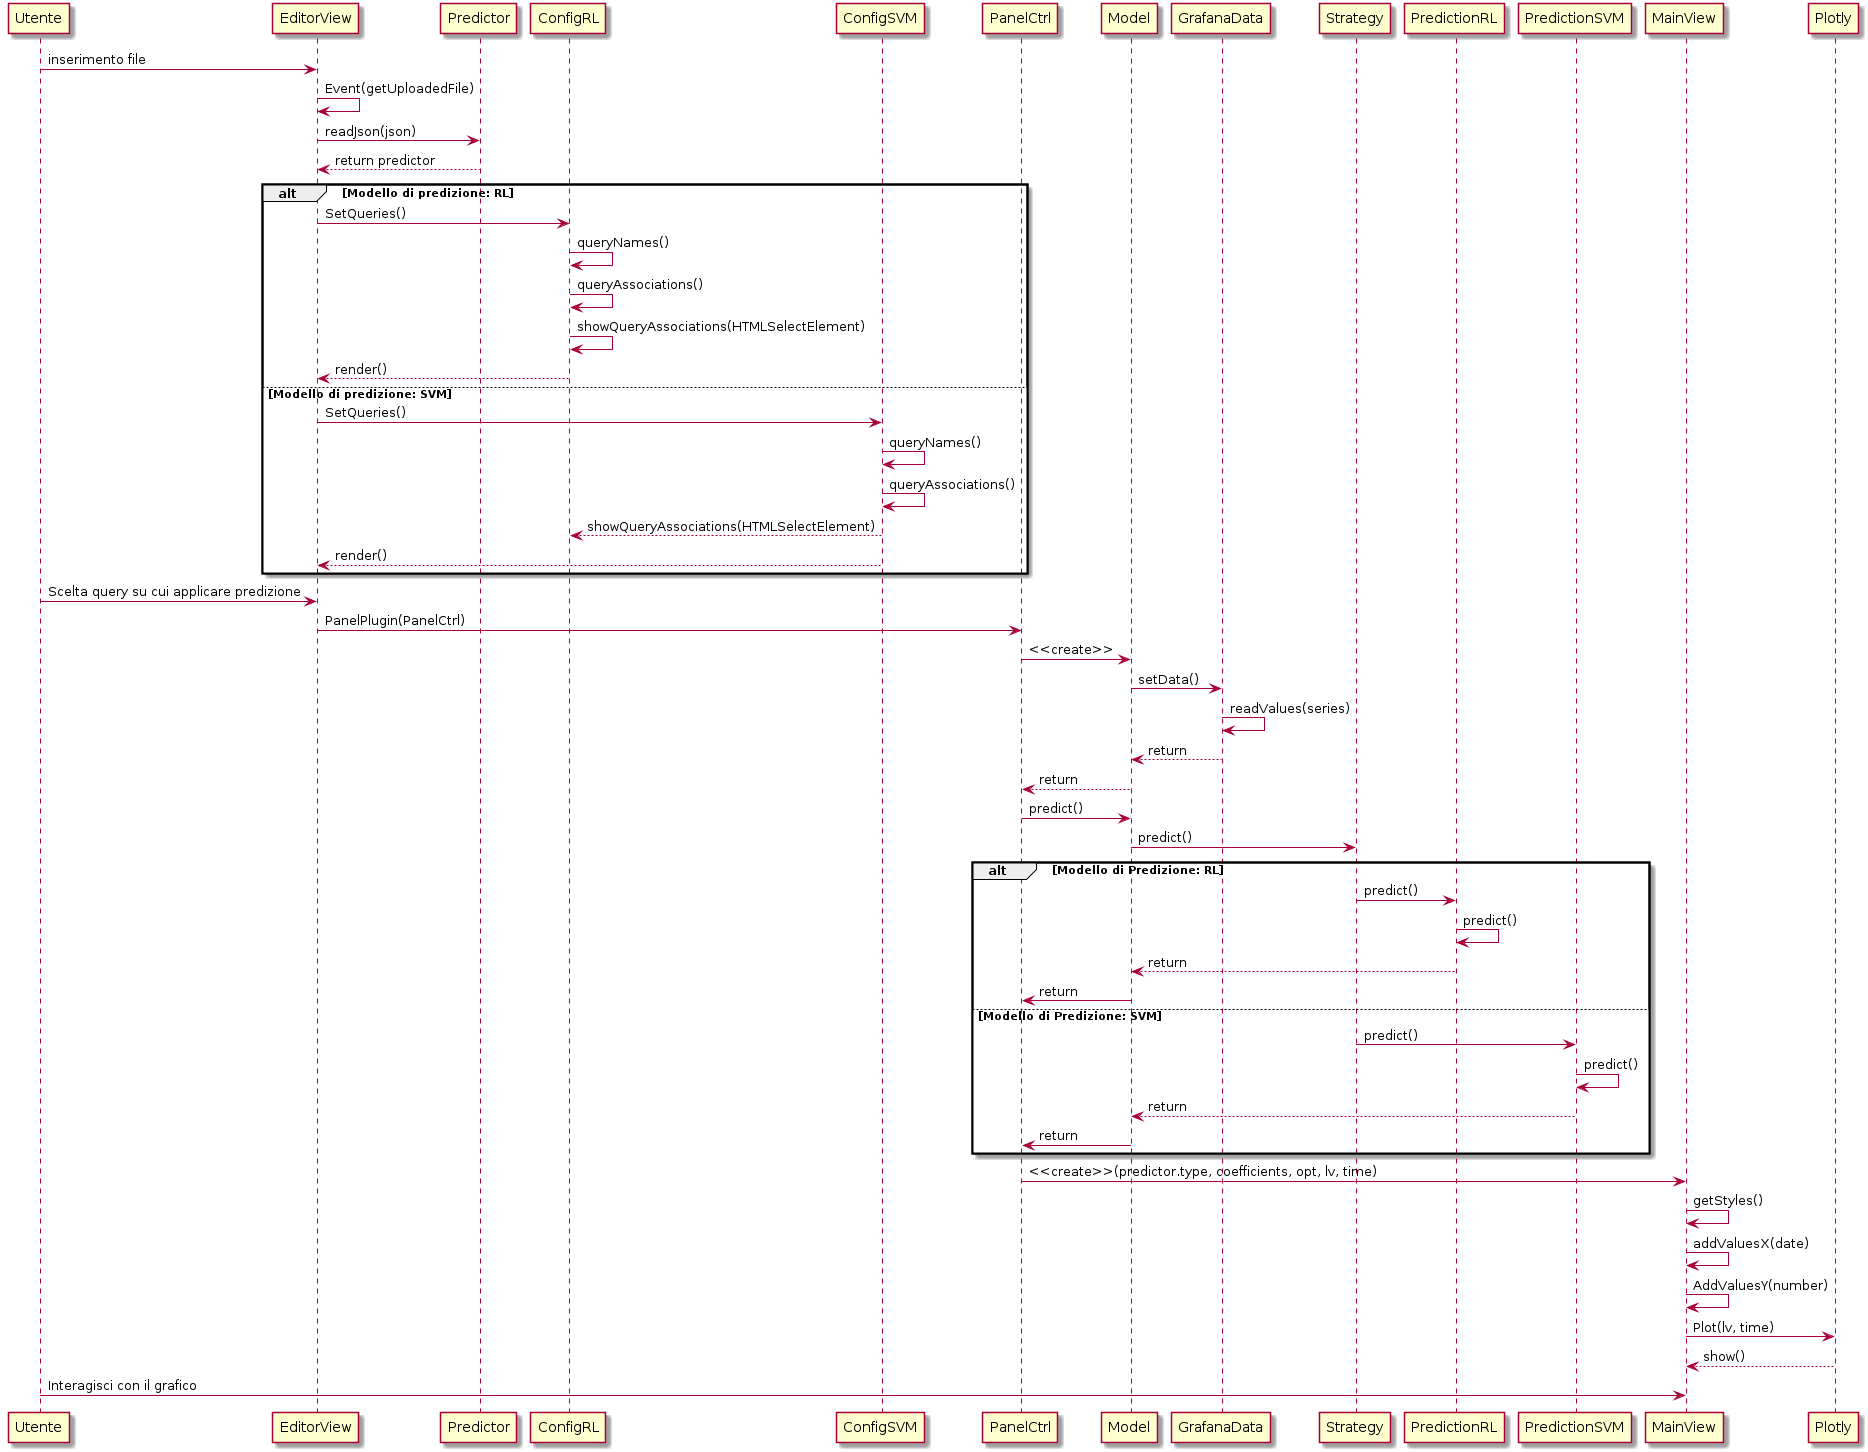
\includegraphics[width=15cm]{img/plugin/sequenceDiagramPlug.png}
  \caption{Diagramma di sequenza del plug-in.}
\end{figure}

\end{document}
